% !TEX root = ../lectures.tex
\section{Nuclei-Proton Interactions}
\label{sec:nucleiproton}

Understanding interactions between nucleons (protons and neutrons) and nuclei is critical for high-energy astrophysics. These interactions are primarily governed by the \emph{strong nuclear force}, a fundamental interaction responsible for binding protons and neutrons within atomic nuclei. This force is characterized by being short-ranged as it operates only over distances comparable to the size of a nucleus (\( \sim 1~\text{fm}\)). 

Unlike point-like elementary particles such as leptons (e.g., electrons) or photons, nucleons and nuclei have an extended spatial structure. The effective size of a nucleus can be approximated by its radius, given by:
\begin{equation}
R_N \sim 1.2 \, A^{1/3} \, \text{fm},
\end{equation}
where \(A\) is the mass number (the total number of protons and neutrons). 

The \emph{geometrical cross-section} is a measure of the probability of interaction between two colliding nuclei or nucleons, based on their physical size:
\(
\sigma_{\rm geom} \simeq \pi R_N^2.
\)

Substituting \(R_N \sim 1.2 \, A^{1/3}~\text{fm}\), we find:
\begin{equation}\label{eq:sgeo}
\sigma_{\rm geom} \simeq \pi (1.2 A^{1/3})^2~\text{fm}^2 \simeq 45 \, A^{2/3}~\text{mb},
\end{equation}
where \(1~\text{mb} = 10^{-27}~\text{cm}^2\). This result implies that larger nuclei (higher \(A\)) have significantly larger cross-sections, increasing their likelihood of undergoing interactions. This approximation provides a useful rule of thumb for estimating nuclear interaction cross-sections~\cite{Letaw1983apjs}. 

The \emph{interaction timescale} is the average time a high-energy particle will travel before interacting with the ambient medium. For a particle propagating through a gas of target particles with number density \(n_{\rm target}\), the timescale is inversely proportional to the product of the cross-section and the speed of the particle:
\begin{equation}
\tau \simeq \frac{1}{n_{\rm target} \sigma_{\rm geom} c}.
\end{equation}

For cosmic-ray protons interacting with hydrogen gas (\(n_{\rm H}\) in \(\text{cm}^{-3}\)), this becomes:
\begin{equation}
\tau \simeq 25 \, A^{-2/3} \left( \frac{n_{\rm H}}{\text{cm}^{-3}} \right)^{-1}~\text{Myr}.
\end{equation}

This equation highlights that in regions with enhanced gas density, such as the inner regions of starburst galaxies or galactic molecular clouds, this interaction timescale becomes comparable to or shorter than other competing processes, such as cosmic-ray escape or energy losses. 
Moreover, \emph{heavier nuclei} have shorter timescales due to their higher cross-sections.

\subsection{Pion Production in Proton-Proton Collisions}

When high-energy protons collide with other protons, the energy in the collision can generate new particles, including pions (\(\pi\)), the lightest mesons. These collisions are the main source of gamma rays and neutrinos in astrophysical environments. 

The primary interactions of high-energy protons with ambient protons produce the following outcomes:
\begin{equation}
p + p \rightarrow 
\begin{cases}
p + p + \pi^0 \\
p + n + \pi^+  \\
p + p + \pi^+ + \pi^-
\end{cases}
\end{equation}
These reactions depend on the energy of the incoming proton. Pions (\(\pi^0, \pi^+, \pi^-\)) are unstable and decay rapidly, leading to secondary particles:

- \emph{Neutral pions} (\(\pi^0\)) decay into gamma rays:
\begin{equation}
\pi^0 \rightarrow \gamma + \gamma.
\end{equation}

- \emph{Charged pions} (\(\pi^\pm\)) decay into muons (\(\mu^\pm\)) and neutrinos:
\begin{equation}
\pi^+ \rightarrow \mu^+ + \nu_\mu, \quad \mu^+ \rightarrow e^+ + \bar{\nu}_\mu + \nu_e,
\end{equation}
\begin{equation}
\pi^- \rightarrow \mu^- + \bar{\nu}_\mu, \quad \mu^- \rightarrow e^- + \nu_\mu + \bar{\nu}_e.
\end{equation}

Thus, each charged pion decay produces \emph{three neutrinos}, while each neutral pion decay produces \emph{two gamma rays}. This simultaneous production of gamma rays and neutrinos is a \emph{distinctive feature of hadronic interactions}.

For pion production to occur, the colliding protons must supply enough energy to create the mass of the pion and satisfy conservation laws. In the LAB frame, the energy threshold \(E_p^{\rm th}\) is determined by~\TODO{add an appendix on thresholds}:
%
\begin{equation}
2 m_p^2 + 2 E^{\rm th}_p m_p = \left(2 m_p + m_{\pi^0} \right)^2,
\end{equation}
%
where \(m_p\) and \(m_{\pi^0}\) are the masses of the proton and neutral pion, respectively. Solving for \(E_p^{\rm th}\), we find:
%
\begin{equation}
E_p^{\rm th} = \frac{(2 m_p + m_{\pi^0})^2 - 2 m_p^2}{2 m_p}.
\end{equation}

Using \(m_p \simeq 0.938~\text{GeV}\) and \(m_{\pi^0} \simeq 0.135~\text{GeV}\), this yields:
\begin{equation}
E_p^{\rm th} \simeq 1.22~\text{GeV}.
\end{equation}

The corresponding \emph{kinetic energy threshold} is:
\begin{equation}
T_p^{\rm th} = E_p^{\rm th} - m_p \simeq 280~\text{MeV}.
\end{equation}

\subsection{Cross-Sections for Proton-Proton Collisions}

\begin{figure}[t] \centering 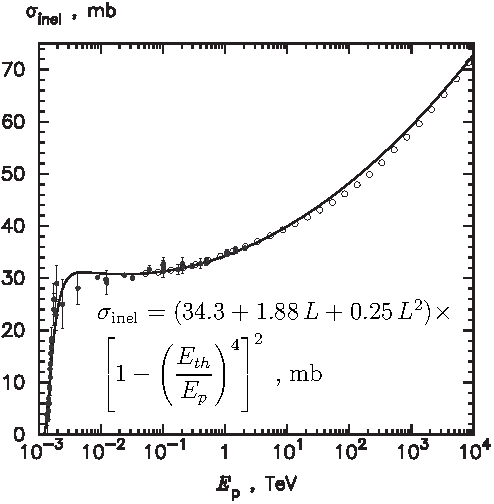
\includegraphics[width=0.5\textwidth]{figures/KelnerAharonian11.pdf} \caption{The energy dependence of the inelastic cross-section for proton-proton collisions, based on the parameterization by Kelner and Aharonian~\cite{Kelner2006prd}.} \label{fig:ppin} \end{figure}

The \emph{inelastic cross-section} \(\sigma_{\rm inel}\) for proton-proton collisions quantifies the probability of interactions where the colliding protons undergo a transformation that produces additional particles, such as pions, in the final state. These interactions typically involve the redistribution of a significant fraction of the initial proton energy among the newly created particles.
%
Experimental measurements indicate that the \emph{inelastic cross-section} \(\sigma_{\rm inel}\) increases rapidly near the pion production threshold (\(T_p \sim 280~\text{MeV}\)) as new particle production becomes possible. It reaches a plateau at several tens of millibarns (\(\sim 30~\text{mb}\)) for proton energies in the GeV range. Beyond a few TeV, \(\sigma_{\rm inel}\) grows more gradually, approximately doubling to \(\sim 60~\text{mb}\) at proton energies on the order of a few PeV.

A useful expression for \(\sigma_{\rm inel}\), valid for \(T_p \gtrsim 1~\text{GeV}\), is given by~\cite{Kelner2006prd}:
\begin{equation}
\sigma_{\rm inel} = (34.3 + 1.88~L + 0.25~L^2) \left[ 1 - \left( \frac{E^{\rm th}_p}{E_p} \right)^4 \right]^2 \, \text{mb},
\end{equation}
where \(L = \ln(E_p / \text{TeV})\). 

\subsection{Inclusive Cross-Sections for Pion Production }

\begin{figure}[t]
\centering
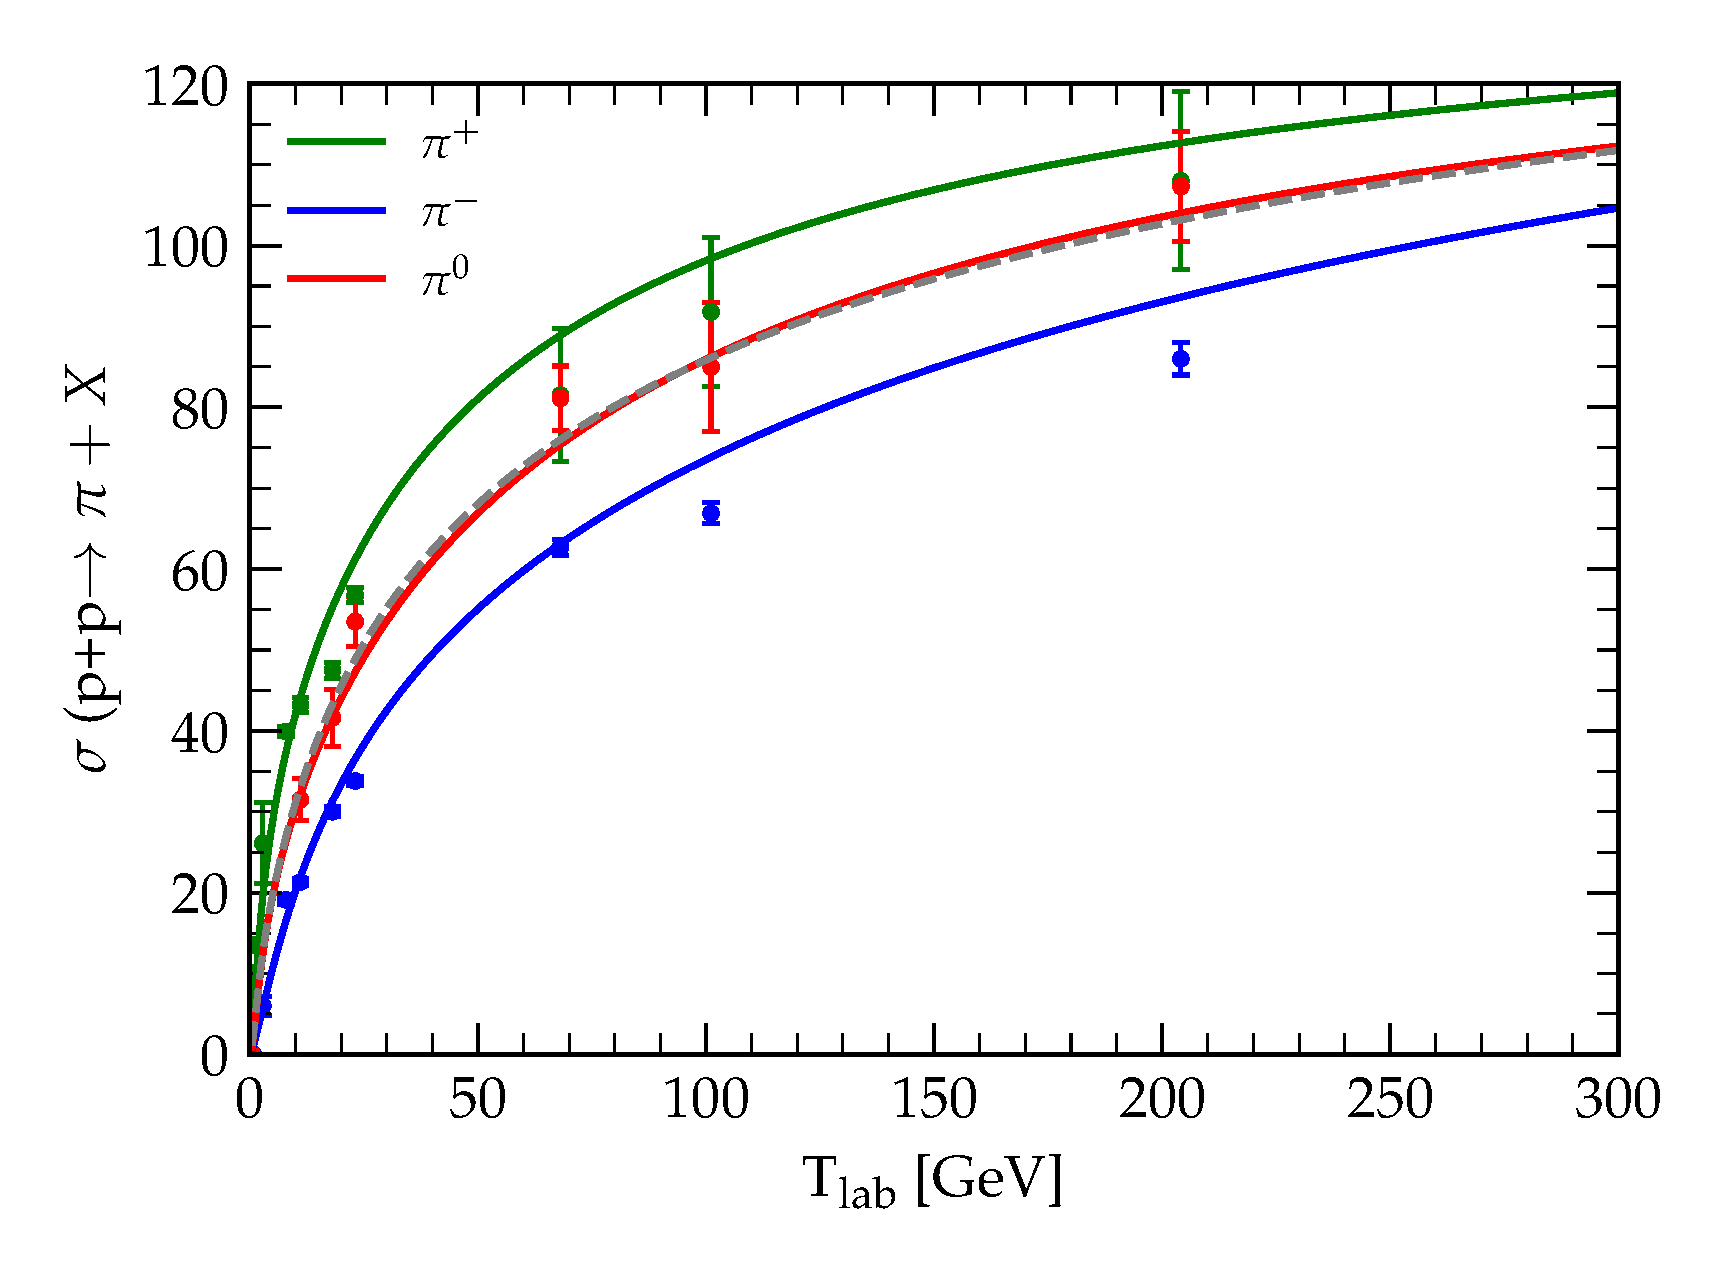
\includegraphics[width=0.5\textwidth]{figures/pion_production.pdf}
\caption{Parameterized inclusive cross sections for pion production in proton-proton collisions~\cite{Norbury2009nimpb}.}
\label{fig:pionprod}
\end{figure}

To describe pion production in proton-proton collisions, \cite{Norbury2009nimpb} provides parameterizations for the \emph{inclusive} cross-sections of \(\pi^+\), \(\pi^-\), and \(\pi^0\) production as functions of the kinetic energy of the incoming proton, \(T_p\), in the LAB frame (in GeV). These parameterizations are expressed as follows:  
\begin{equation}
\sigma_{pp \rightarrow \pi^+ X} = \left( 0.00717 + 0.0652 \frac{\log T_p}{T_p} + \frac{0.162}{T_p^2} \right)^{-1}~\text{mb}, 
\end{equation}
\begin{equation}
\sigma_{pp \rightarrow \pi^- X} = \left( 0.00456 + \frac{0.0846}{T_p^{0.5}} + \frac{0.577}{T_p^{1.5}} \right)^{-1}~\text{mb}, 
\end{equation}
\begin{equation}
\sigma_{pp \rightarrow \pi^0 X} = \left( 0.007 + 0.1 \frac{\log T_p}{T_p} + \frac{0.3}{T_p^2} \right)^{-1}~\text{mb}.
\end{equation}  

These equations provide approximate fits to experimental data and are particularly useful for modeling pion production in astrophysical scenarios. The cross-sections are plotted in~\ref{fig:pionprod}, as a function of \(p_{\rm lab}\), the momentum of the incoming proton in the LAB frame~\TODO{rifare il plot}.  

The term \emph{inclusive cross-section} refers to the total probability of a specific outcome in a reaction, summed over all possible accompanying final states. In the context of proton-proton collisions, an inclusive cross-section for pion production, such as \(\sigma_{pp \rightarrow \pi^+ X}\), represents the cross-section for producing a \(\pi^+\) meson, regardless of what other particles (\(X\)) may also be produced in the final state.  

This is in contrast to \emph{exclusive cross-sections}, which describe the probability of a very specific final state, such as \(p + p \rightarrow p + n + \pi^+\). Exclusive cross-sections require detailed knowledge of all the final particles and their properties, whereas inclusive cross-sections provide a comprehensive description of a particular secondary particle's production.  

A key feature of the parameterized cross-sections is their threshold behavior. The production of charged pions, such as \(\pi^+\) and \(\pi^-\), requires a minimum proton kinetic energy, \(T_p\), to satisfy conservation of energy and momentum. For example, the threshold for \(\pi^+\) production is \(T_p \simeq 289~\text{MeV}\). Notably, the threshold for \(\pi^-\) production is higher, \(T_p \simeq 600~\text{MeV}\), due to the presence of two new particles in the final state (e.g., \(\pi^-\) and \(\pi^+\)).  
%
This difference in thresholds leads to a consistently larger cross-section for \(\pi^+\) compared to \(\pi^-\) at all energies above the threshold.  

Neutral pions (\(\pi^0\)), which decay into gamma rays, have a cross-section \(\sigma_{pp \rightarrow \pi^0 X}\) that satisfies the approximate relationship:
%
\begin{equation}
\sigma_{pp \rightarrow \pi^0 X} \simeq \frac{1}{2} \left( \sigma_{pp \rightarrow \pi^+ X} + \sigma_{pp \rightarrow \pi^- X} \right).
\end{equation}
%
This relationship is a reflection of the isospin symmetry of the strong interaction, which predicts a balanced production of charged and neutral pions at high energies.  

The asymmetry in the production cross-sections of \(\pi^+\) and \(\pi^-\) has significant astrophysical consequences. Charged pion decays ultimately lead to the production of secondary leptons, as \(\pi^+ \) (\(\pi^- \)) decays produce positrons (electrons) via \(\mu^+\) (\(\mu^-\)) decay.  
%
Because \(\pi^+\) production dominates over \(\pi^-\) production, cosmic-ray interactions result in an excess of secondary positrons compared to electrons. This excess is an important diagnostic for understanding hadronic processes in astrophysical environments~\cite{Moskalenko1998apj}.  

\subsection{Pion Emissivity and Gamma-Ray Spectrum}

%Pion emissivity is critical for understanding secondary particle production, as the decay of these pions generates gamma rays and neutrinos, key observables in high-energy astrophysics.  

The \emph{pion emissivity}, \(q_\pi(E_\pi)\), represents the number of pions produced per unit volume, time, and energy in a given astrophysical environment.
%
In a medium with a target number density \(n_{\rm H}\), the emissivity can be expressed as:
\begin{equation}\label{eq:qpi}
q_\pi(E_\pi) = c n_{\rm H} \int \delta(T_\pi - K_\pi T_p) \, \sigma_{pp}(E_p) \, N_p(E_p) \, dE_p,
\end{equation}
%
where \(N_p(E_p)\) is differential number density of protons as a function of energy \(E_p\).
%
The factor \(K_\pi\) is a dimensionless constant called the \emph{inelasticity}. It quantifies the \emph{average} fraction of the initial proton's energy lost during the interaction and transferred to the produced pions. For pion production in proton-proton collisions in the GeV-TeV range, the inelasticity is approximately \( K_\pi \simeq 0.17 \)~.

% and \(K_\pi\) is the \emph{inelasticity factor}, representing the fraction of the proton's kinetic energy transferred to the pion.

The delta function, \(\delta(T_\pi - K_\pi T_p)\), is used to approximate the relationship between the energy of the outgoing pion (\(T_\pi\)) and the energy of the incoming proton (\(T_p\)) assuming that the kinetic energy of the outgoing pion is a \emph{fixed} fraction (\(K_\pi\)) of the kinetic energy of the incoming proton:
\( T_\pi \simeq K_\pi T_p \).

Performing the integration in~\ref{eq:qpi} yields:
%
\begin{equation}
q_\pi (E_\pi) \simeq \frac{c n_{\rm H}}{K_\pi} \sigma_{pp} \left(\frac{T_\pi}{K_\pi} + m_p \right) N_p \! \left(\frac{T_\pi}{K_\pi} + m_p \right).
\end{equation}

In the high-energy limit, where the energy of the pion significantly exceeds its rest mass (\(E_\pi \gg m_\pi\)), the contribution of the pion’s mass can be neglected. In this regime, the expression for the pion emissivity simplifies to:
%
\begin{equation}
q_\pi (E_\pi) \simeq \frac{c n_{\rm H}}{K_\pi} \sigma_{pp} \left( \frac{E_\pi}{K_\pi} \right) N_p \left( \frac{E_\pi}{K_\pi} \right).
\end{equation}

From the above result, it becomes evident that the spectrum of the produced pions closely resembles the spectrum of the parent protons, but with a characteristic energy shift by a factor of \(K_\pi\).  

This behavior can be summarized as:
%
\begin{itemize}
\item The pion energy is proportional to the proton energy, scaled by \(K_\pi\).  
\item If the proton spectrum follows a power-law form, \(N_p(E_p) \propto E_p^{-\alpha}\), the pion spectrum will also follow a power law with the same spectral index as \( q_\pi(E_\pi) \propto E_\pi^{-\alpha} \).
\end{itemize}

\subsection{The \(\pi^0\) Gamma-Ray Spectrum }

The decay of a neutral pion (\(\pi^0\)) into two gamma photons is an essential process in high-energy astrophysics, as it provides a direct link between hadronic interactions and observable gamma-ray spectra. The decay occurs via the reaction:  
\begin{equation}
\pi^0 \rightarrow \gamma + \gamma.
\end{equation}  
This decay is extremely fast, with a mean lifetime of approximately \(8.4 \times 10^{-17}\) seconds, meaning the pion effectively decays immediately after production.  

In the \emph{CoM frame} of the pion, momentum conservation ensures that the two photons are emitted in opposite directions (back-to-back). Energy conservation dictates that the energy of each photon is half the rest energy of the pion:
\begin{equation}
E_\gamma^\prime = \frac{m_\pi}{2},
\end{equation}
where \(m_\pi \simeq 135~\text{MeV}\) is the rest mass of the neutral pion.  

In the \emph{LAB frame}, where the pion is moving with velocity \(\beta_\pi = v_\pi / c\), the energies of the photons are modified due to relativistic effects. The photon energy in the LAB frame, \(E_\gamma\), depends on the angle \(\theta^\prime\) between the photon direction in the CoM frame and the direction of the pion's motion. 
%
Using relativistic energy transformations, we find:
\begin{equation}\label{eq:egammaboost}
E_\gamma = \frac{m_\pi}{2} \gamma_\pi (1 + \beta_\pi \cos \theta^\prime),
\end{equation}
where \(\gamma_\pi = (1 - \beta_\pi^2)^{-1/2}\) is the Lorentz factor of the moving pion,  and \(\theta^\prime\) is the angle of emission in the pion’s CoM frame.  
%
This equation captures the fact that photons emitted in the direction of the pion's motion (\(\cos \theta^\prime = +1\)) are blueshifted, while those emitted in the opposite direction (\(\cos \theta^\prime = -1\)) are redshifted.  

To find the range of photon energies in the LAB frame, we vary \(\cos \theta^\prime\) from \(-1\) to \(+1\). This gives the extreme photon energies as:
\begin{equation}\label{eq:gammaminmax}
E_\gamma^{\rm min/max} = \frac{m_\pi}{2} \gamma_\pi (1 \mp \beta_\pi),
\end{equation}

In the non-relativistic limit, the pion’s motion is negligible (\(\gamma_\pi \simeq 1\)), and the photon energies converge to the same value 
\begin{equation} 
E_\gamma^{\rm min} \simeq E_\gamma^{\rm max} \simeq \frac{m_\pi}{2}.
\end{equation}

Conversely, in the ultra-relativistic limit, the pion moves close to the speed of light, and \(\gamma_\pi \gg 1\). In this case the maximum photon energy approaches the total pion energy \( E_\gamma^{\rm max} \simeq E_\pi \), while the minimum photon energy becomes arbitrarily small \( E_\gamma^{\rm min} \simeq 0 \)~.

%These behaviors reflect the highly anisotropic photon distribution in the LAB frame for ultra-relativistic pions, with most photon energy concentrated in the forward direction.

The relationship between the photon energy and the emission angle in the LAB frame can be further analyzed. From the LAB-frame energy in~\ref{eq:egammaboost}, we can compute the differential relationship between photon energy and the cosine of the angle:
\begin{equation}\label{eq:degamma}
dE_\gamma = \frac{m_\pi}{2} \gamma_\pi \beta_\pi \, d\!\cos \theta^\prime.
\end{equation}

Since the pion is a scalar particle (spin-0), its decay products are emitted isotropically in the pion’s rest frame. This isotropic emission is expressed mathematically as:
\begin{equation}
\int d\Omega \frac{dN_\gamma}{d\Omega} = 1,
\end{equation}
where \(\frac{dN_\gamma}{d\Omega}\) represents the probability distribution of photon emission over solid angle \(d\Omega\).  
%
Thus, the isotropic photon distribution becomes
\begin{equation}
\frac{dN_\gamma}{d\Omega} = \frac{1}{4\pi},
\end{equation}
%
and the differential number of photons emitted in a given angular range \(d\cos\theta^\prime\) is~\footnote{Using the relation \(d\Omega = \sin \theta d\theta d\phi\) and averaging over the azimuthal angle \(\phi\), the solid angle simplifies to \(\langle d\Omega \rangle_\phi = 2\pi d\cos\theta\).}:
\begin{equation}\label{eq:dngammadcos}
dN_\gamma = \frac{1}{2} \, d\cos\theta^\prime.
\end{equation}

Combining the derivative of \(E_\gamma\) with respect to \(\cos \theta^\prime\) from~\ref{eq:degamma} with the isotropic emission result in~\ref{eq:dngammadcos}, the photon energy distribution can be expressed as:
%
\begin{remark}
\begin{equation}
\frac{dN_\gamma}{dE_\gamma} = \frac{1}{m_\pi \gamma_\pi \beta_\pi} = \frac{1}{(E_\pi^2 - m_\pi^2)^{1/2}}~.
\end{equation}
\end{remark}
%
Thus, for fixed pion energy, the photon energies are \emph{uniformly} distributed between \(E_\gamma^{\rm min}\) and \(E_\gamma^{\rm max}\), leading to a \emph{box-like spectrum} of gamma rays.  

To characterize this box-like distribution, we calculate the central energy in logarithmic space:
\begin{equation}
\langle \log E_\gamma \rangle = \frac{1}{2} \left( \log E_{\gamma, \rm min} + \log E_{\gamma, \rm max} \right).
\end{equation}

Substituting~\ref{eq:gammaminmax}, and simplifying using \(\gamma_\pi^2 - 1 = \beta_\pi^2 \gamma_\pi^2\), we find:
\begin{remark}
\begin{equation}
\langle \log E_\gamma \rangle 
= \log \left[ \frac{E_\pi^2}{4} (1-\beta_\pi^2) \right]^{1/2} 
=\log \left( \frac{m_\pi}{2} \right).
\end{equation}
\end{remark}

This result shows that the logarithmic central energy of the spectrum is fixed at half the pion mass (\(m_\pi / 2 \simeq 67.5~\text{MeV}\)), independent of the pion's energy \(E_\pi\).

\begin{figure}[t]
\centering
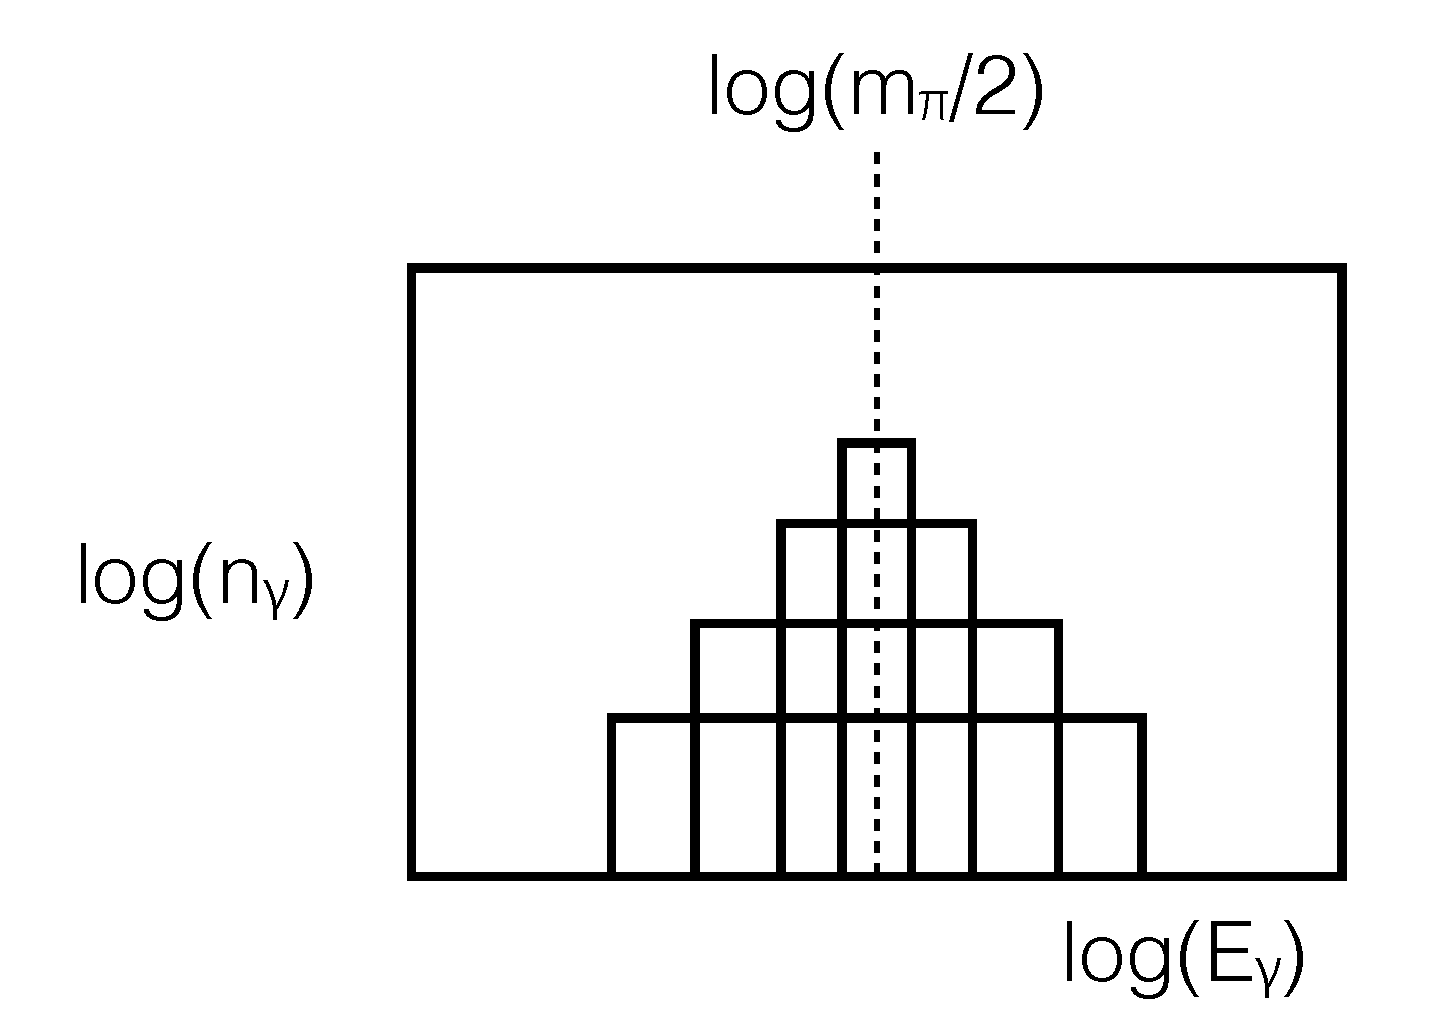
\includegraphics[width=0.5\textwidth]{figures/pion_bump.png}
\caption{Pion bump~\TODO{add credits}.}
\label{fig:pionbump}
\end{figure}

Assuming a distribution of pion energies, the resulting gamma-ray spectrum is composed of a weighted sum of individual \emph{box-like} distributions. Each box-like distribution is symmetrically centered in logarithmic space around \(m_\pi / 2\), which corresponds to the logarithmic central energy of the photons produced in the pion's rest frame. As a result, the combined gamma-ray spectrum exhibits a clear peak at \( \log E_\gamma \simeq \log \left(\frac{m_\pi}{2}\right) \)~(see \ref{fig:pionbump}).  

This spectral feature, often referred to as the \emph{pion bump}, is a prominent characteristic of gamma rays originating from hadronic processes. The bump appears at \(\sim 70~\text{MeV}\), followed by a decline at higher energies, and is largely independent of the underlying pion spectrum or the spectrum of the parent protons.  

Such a bump-like structure in the gamma-ray spectrum, combined with its distinct position and shape, provides a strong diagnostic tool for identifying gamma rays resulting from hadronic interactions (see \ref{fig:pionbumpfermi}).  

\begin{figure}[!t]
\centering
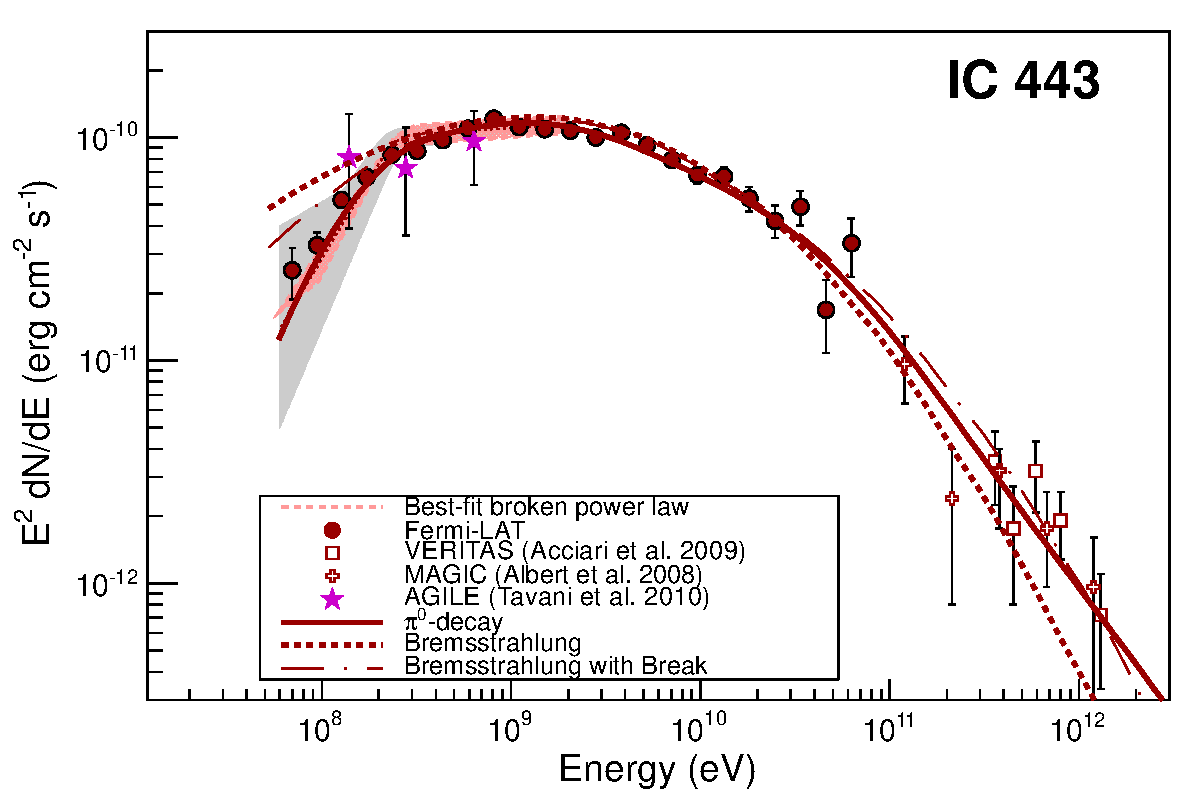
\includegraphics[width=0.45\textwidth]{figures/1231160fig2a.pdf}
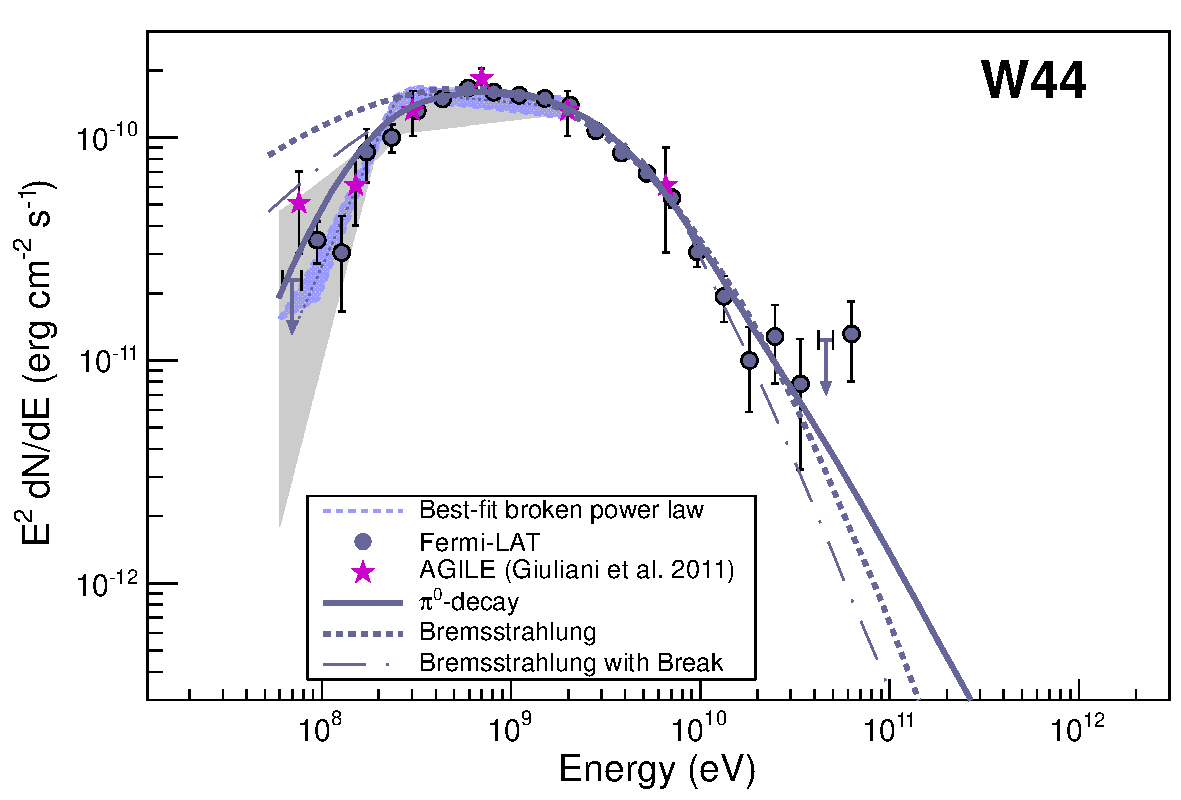
\includegraphics[width=0.45\textwidth]{figures/1231160fig2b.pdf}
\caption{In 2013 FERMI detected a feature compatible with the pion-bump in two old SNRs in interaction with Molecular Cloud~\cite{Ackermann2013sci}}
\label{fig:pionbumpfermi}
\end{figure}

\subsection{Gamma-Ray Emissivity}

The gamma-ray emissivity, \(q_\gamma(E_\gamma)\), describes the production rate of gamma rays with energy \(E_\gamma\) per unit time, volume, and energy. It is derived from the pion emissivity, \(q_\pi(E_\pi)\), by summing the contributions from all pions capable of producing gamma photons with energy \(E_\gamma\). This is expressed as:
\begin{equation}
q_\gamma(E_\gamma) = 2 \int_{E_{\pi, \rm min}}^\infty dE_\pi \, q_\pi(E_\pi) \frac{dN}{dE_\gamma},
\end{equation}
where the factor of 2 accounts for the two photons emitted in each \(\pi^0\) decay,  \(E_{\pi, \rm min}\) is the minimum pion energy required to produce a photon of energy \(E_\gamma\), and \(\frac{dN}{dE_\gamma}\) represents the energy distribution of photons from a pion of energy \(E_\pi\).  

To determine the minimum pion energy \(E_{\pi, \rm min}\) needed to produce a photon of energy \(E_\gamma\), we notice that the photon energies in the LAB frame are bounded by \( E_{\gamma, \rm min} + E_{\gamma, \rm max} = E_\pi \), and \( E_{\gamma, \rm min} E_{\gamma, \rm max} = \frac{m_\pi^2}{4} \).

These two relations can be combined to express the pion energy in terms of \(E_{\gamma, \rm max}\):
\begin{equation}
E_\pi = E_{\gamma, \rm min} + E_{\gamma, \rm max} = \frac{m_\pi^2}{4 E_{\gamma, \rm max}} + E_{\gamma, \rm max}.
\end{equation}

For a photon of energy \(E_\gamma\), the minimum pion energy \(E_{\pi, \rm min}\) occurs when \(E_{\gamma, \rm max} = E_\gamma\), as this corresponds to the highest-energy photon being emitted directly along the pion’s direction of motion. Therefore, we find:
%
\begin{equation}
E_{\pi, \rm min} = E_\gamma + \frac{m_\pi^2}{4 E_\gamma}.
\end{equation}

Using this, the gamma-ray emissivity becomes:
%
\begin{remark}
\begin{equation}\label{eq:qgamma2}
q_\gamma(E_\gamma) = 2 \int_{E_\gamma + \frac{m_\pi^2}{4 E_\gamma}}^\infty dE_\pi \frac{q(E_\pi)}{(E_\pi^2 - m_\pi^2)^{1/2}} \oset{E_\gamma \gg m_\pi}{\simeq} 2 \int_{E_\gamma}^\infty \frac{dE_\pi}{E_\pi} q_\pi(E_\pi)
\end{equation}
\end{remark}
%
where the final expression holds true at high energies where the pion mass can be considered negligible.

This simplified expression highlights an important feature of the gamma-ray spectrum at high energies! The gamma-ray spectrum \( q_\gamma(E_\gamma) \) is directly linked to the pion spectrum, retaining the same spectral index.
Since the pion spectrum itself mirrors the parent proton spectrum at high energies, the gamma-ray spectrum ultimately inherits the spectral index of the cosmic-ray protons, \( E_\gamma^{-\alpha_p} \).

The only modification is a shift in energy due to the inelasticity factor, with gamma rays appearing at an energy scale approximately \( K_\gamma = K_\pi / 2 \) times the energy of the parent protons.

This behavior contrasts sharply with that of gamma rays generated by IC scattering, where the spectral index of the gamma rays reflects a different scaling relative to the parent electron spectrum. In particular, for IC scattering, the gamma-ray spectrum tends to exhibit a comparatively flatter dependence on energy, scaling approximately as \(E_\gamma^{-(\alpha_e+1)/2}\), where \(\alpha_e\) is the spectral index of the electron spectrum.  

This distinction is crucial for disentangling the origin of high-energy gamma rays in astrophysical observations. While gamma rays from hadronic processes closely mirror the spectral index of cosmic-ray protons, those produced via IC scattering from relativistic electrons typically show a softer or flatter spectrum.

\subsection{Diffuse Galactic Gamma-Ray Emission}

In this section, we explore a significant application of the gamma-ray emissivity calculation by addressing the diffuse gamma-ray emission resulting from galactic cosmic rays interacting with interstellar matter. Cosmic rays, primarily protons, traverse the interstellar medium and interact with ambient gas, producing pions that decay into gamma rays. By moving beyond the delta-function approximation, we calculate the pion emissivity as follows:  
%
\begin{equation}
q(E_\pi) = c n_{\rm H} \int_{E_\pi}^\infty dE_p \, N_p(E_p) \frac{d\sigma}{dE_\pi}(E_p, E_\pi) = 4 \pi n_{\rm H} \int_{E_\pi}^\infty dE_p \, I_p(E_p) \frac{d\sigma}{dE_\pi}(E_p, E_\pi),
\end{equation}
%
where \(\frac{d\sigma}{dE_\pi}(E_p, E_\pi)\) is the \emph{differential pion production cross-section}, and \(N_p(E_p) \) is the proton density per unit of energy.  
%
We conveniently convert the proton density \(N_p(E_p) \) to the proton intensity \( I_p(E_p) \) defined as \( I_p(E_p) =  \frac{c}{4\pi} N_p(E_p) \) as this is the quantity typically provided by measurements.

The differential cross-section \(\frac{d\sigma}{dE_\pi}\) for pion production in proton-proton interactions can be parameterized in terms of the \emph{total inclusive cross-section} \(\sigma_{pp}\) and a normalized auxiliary function \(f(E_p, E_\pi)\), designed to fit experimental data:  
\begin{equation}
\frac{d\sigma}{dE_\pi}(E_p, E_\pi) = \sigma_{pp}(E_p) \frac{f(E_p, E_\pi)}{E_\pi} \simeq \sigma_0 \frac{f(E_p, E_\pi)}{E_\pi}.
\end{equation}

The function \(f(E_p, E_\pi)\) describes the energy distribution of the produced pions, and it has been observed that it primarily depends on the ratio \(x = E_\pi / E_p\).
%
A widely used parameterization of \(f(x)\) is given by~\cite{Berezinskii1988sal}:
\begin{equation}
f(x) = 0.67 (1-x)^{3.5} + 0.5 \exp(-18x),
\end{equation}
where \(x \in [0, 1]\).  

Finally, we approximate the inelastic cross-section as a constant, using its plateau value at \( \gtrsim \)~GeV energy: \( \sigma_{pp} \sim \sigma_0 \simeq 30 \)~mbarn.

%with the normalization condition:
%\begin{equation}
%\int_{E_{\pi, \rm min}}^{E_{\pi, \rm max}} \frac{dE_\pi}{E_\pi} f(E_p, E_\pi) = 1.
%\end{equation}

The observed proton intensity in cosmic rays, \(I_p(E_p)\), is generally well-represented by a power-law spectrum:
\begin{equation}
I_p(E_p) = I_{10} \left(\frac{E_p}{E_{10}}\right)^{-\alpha},
\end{equation}
where \(I_{10}\) is the proton intensity at a reference energy \(E_{10} = 10~\text{GeV}\), and \(\alpha \sim 2.7\) is the spectral index.  

Substituting this form and the parameterization for \(\frac{d\sigma}{dE_\pi}\) into the expression for \(q(E_\pi)\), we obtain:
\begin{equation}
q(E_\pi) \simeq 4 \pi n_{\rm H} I_{10} \sigma_0 \int_{E_\pi}^\infty \frac{dE_p}{E_\pi} \left(\frac{E_p}{E_{10}} \right)^{-\alpha} f(x).
\end{equation}

Changing the integration variable to \(x = E_\pi / E_p\), the emissivity simplifies to:
\begin{equation}
q(E_\pi) = 4 \pi n_{\rm H} I_{10} \sigma_0 \left(\frac{E_\pi}{E_{10}} \right)^{-\alpha} \underbrace{\int_0^1 dx \, x^{\alpha-2} f(x)}_{Y(\alpha)},
\end{equation}
where \(Y(\alpha)\) is the \emph{spectrum-weighted yield of pions} produced from a proton population with a power-law spectral index \(\alpha\).  

The photon emissivity \(q_\gamma(E_\gamma)\) can now be calculated from~\ref{eq:qgamma2}:  
\begin{equation}
q_\gamma(E_\gamma) = 8 \pi n_{\rm H} \sigma_0 Y(\alpha) I_{10} \int_{E_\gamma}^\infty \frac{dE_\pi}{E_\pi} \left(\frac{E_\pi}{E_{10}}\right)^{-\alpha}.
\end{equation}

Performing the integration yields:
\begin{equation}
E_\gamma^2 q_\gamma(E_\gamma) = \frac{8 \pi}{\alpha} n_{\rm H} \sigma_0 Y(\alpha) E_{10}^2 I_{10} \left(\frac{E_\gamma}{E_{10}}\right)^{2-\alpha}.
\end{equation}

Using the gamma-ray emissivity \(q_\gamma(E_\gamma)\), we can estimate the diffuse gamma-ray intensity arising from proton-proton interactions in the Galactic plane. Assuming a uniform distribution of cosmic rays and interstellar gas, the gamma-ray intensity along a line of sight (los) is given by:
\begin{equation}
I_\gamma(E_\gamma) = \frac{1}{4\pi} \int_{\rm los} ds \, q_\gamma(E_\gamma).
\end{equation}

Substituting \(q_\gamma(E_\gamma)\) and defining the gas column density as \(N_{\rm H} = \int_{\rm los} ds \, n_{\rm H}\), we find:
\begin{remark}
\begin{equation}
E_\gamma^2 I_\gamma = \frac{2}{\alpha} N_{\rm H} \sigma_0 Y(\alpha) E_{10}^2 I_p(E_{10}) \left(\frac{E_\gamma}{E_{10}}\right)^{2-\alpha}.
\end{equation}
\end{remark}

To estimate the gamma-ray intensity at \(E_\gamma = 1~\text{GeV}\) we adopt:  
%
\begin{itemize}
\item The gas column density along the Galactic plane is approximately \(N_{\rm H} \simeq 10^{22}~\text{cm}^{-2}\)~\cite{addref}.  
\item The observed proton intensity at \(E_p = 10~\text{GeV}\) is \(E_{10}^2 I_p(E_{10}) \simeq 0.2~\text{GeV}~\text{cm}^{-2}~\text{s}^{-1}~\text{sr}^{-1}\)~\cite{crdb} 
\item For \(\alpha \simeq 2.7\), we compute the yield as \(Y(\alpha) \simeq 4 \times 10^{-2}\).
\end{itemize}

Substituting these values, we find:
\begin{equation}
E_\gamma^2 I_\gamma \simeq 10^{-5}~\text{GeV}~\text{cm}^{-2}~\text{s}^{-1}~\text{sr}^{-1}.
\end{equation}

This value aligns well with observations of the diffuse gamma-ray emission measured by Fermi-LAT along the Galactic plane (\(|b| < 5^\circ\)) at \(E_\gamma \simeq 1~\text{GeV}\)~\cite{addref}.  

This result strongly supports the hypothesis that the diffuse galactic gamma-ray emission originates from the interactions of the (approximately uniform) cosmic rays  with interstellar gas, predominantly through proton-proton collisions, with a spectrum reflecting the underlying cosmic-ray proton spectrum.

\begin{problem}
Compute the shape of $q_\gamma(E_\gamma)$ using the fitting formula of Eq.~(1) in 1302.3307 and using the $\delta$-function approximation. Plot $q_\gamma(E_\gamma)$ in linear scale and $E_\gamma^2q_\gamma(E_\gamma)$ in log-log one. 
\end{problem}

\section{Nuclei-\(\gamma\) Interactions}

In astrophysical environments, dense radiation fields are often present near energetic sources such as active galactic nuclei (AGN), gamma-ray bursts (GRBs), and supernova remnants. These radiation fields can significantly influence the propagation and energy loss mechanisms of cosmic rays.  

While the cross-section for \(\gamma\)-proton interactions is typically about two orders of magnitude smaller than that of proton-proton (\(pp\)) interactions, certain environments exhibit a much higher photon number density, \(n_\gamma\), compared to the matter density. As a result, \emph{photoproduction processes} can dominate over \(pp\) interactions in these scenarios.  

\subsection{Photo-Pion Production}

The dominant mechanism in the interaction of nuclei with radiation fields is \emph{photo-pion production}, which involves the creation of pions via interactions between high-energy protons and photons. The key reaction pathway is: 
\begin{equation}\label{eq:deltares}
p + \gamma \rightarrow \Delta^+ \rightarrow
\begin{cases}
p + \pi^0, & \text{(neutral pion production)} \\
n + \pi^+, & \text{(charged pion production)} 
\end{cases}
\end{equation}
%
where \(\Delta^+\) is an intermediate baryon resonance state with a lifetime of \( \sim 10^{-23} \) seconds.  

The decay of the neutral pion (\(\pi^0\)) produces gamma rays, while the charged pion (\(\pi^\pm\)) decays into neutrinos and leptons as discussed in the previous section.

At very high proton energies, \emph{multi-pion production} becomes significant, represented schematically as:
\begin{equation}
p + \gamma \rightarrow p + a \pi^0 + b (\pi^+ + \pi^-),
\end{equation}
where \(a\) and \(b\) represent the multiplicities of neutral and charged pions, respectively. 
%
Multi-pion production becomes increasingly relevant as the energy of the interacting proton increases.  

\subsection{Pair Production}

Another energy-loss mechanism for high-energy cosmic rays in radiation fields is \emph{pair production}, which produces electron-positron pairs:  
\begin{equation}
p + \gamma \rightarrow p + e^+ + e^-~.
\end{equation}  

While this process generally involves smaller energy losses compared to photo-pion production, it is still a competitive energy-loss channel for protons in certain astrophysical environments as it requires a smaller energy threshold.  

\subsection{Energy Thresholds}

The energy thresholds for these interactions can be calculated based on energy and momentum conservation laws~\cite{appendix}. These thresholds depend on two key factors: the energy of the target photon (\(\epsilon\)) in the LAB frame and the angle \(\theta\) between the momenta of the proton and the photon.  

In extragalactic space, the most abundant photon field is the cosmic microwave background (CMB), characterized by a mean photon energy of \(\epsilon \sim 10^{-4}\)~eV. Under these conditions:  

For photo-pion production, the threshold energy for a proton to produce pions via interaction with a photon is:  
\begin{equation}
E_p^\pi = \frac{m_\pi^2 + 2 m_\pi m_p}{2 \epsilon (1 - \cos \theta)},
\end{equation}

Substituting typical CMB photon energies and assuming head-on collisions (\(1 - \cos \theta \sim 2\)), we find:
\begin{equation}
E_p^\pi \simeq 7 \times 10^{9}~\text{GeV}.
\end{equation}

For pair production, the threshold energy for a proton to produce an electron-positron pair via interaction with a photon is:  
\begin{equation}
E_p^{ee} = \frac{4 m_e^2 + 8 m_e m_p}{2 \epsilon (1 - \cos \theta)},
\end{equation}

Substituting the same conditions for the CMB, we find:
\begin{equation}
E_p^{ee} \simeq 6 \times 10^{17}~\text{eV}.
\end{equation}

Both threshold energies are inversely proportional to the photon energy (\(\epsilon\)), meaning that interactions with higher-energy photon fields  require lower proton energies to satisfy the threshold condition. 

\subsection{Photo-Pion Production Cross-Section}

The cross-section for photo-pion production has been well-measured in laboratory experiments. It peaks in the \(\Delta^+\)-resonance region and decreases at higher photon energies. The approximate behavior is:  
%
\begin{equation}
\sigma_{p\gamma} \simeq 
\begin{cases}
340 \, \mu\text{b}, & 200 \, \text{MeV} \lesssim E_\gamma^\prime \lesssim 500 \, \text{MeV}, \\
120 \, \mu\text{b}, & E_\gamma^\prime \gtrsim 500 \, \text{MeV},
\end{cases}
\end{equation}
%
where \(E_\gamma^\prime\) is the photon energy in the proton’s rest frame.  

The \emph{inelasticity} of the photo-pion production process, representing the fraction of energy lost by the proton per interaction, is approximately \(K_{p\gamma} \simeq 0.2\).  

The \emph{cooling timescale} for protons losing energy via photo-pion production can be estimated as:  
%
\begin{equation}
t_c(E) \simeq \frac{E}{\dot{E}} \sim \frac{\Delta t}{\Delta E / E} \sim \frac{1}{K_{p\gamma} n_\gamma c \sigma_{p\gamma}} \sim 44 \left( \frac{n_\gamma}{400~\text{cm}^{-3}} \right)^{-1}~\text{Myr}
\end{equation}
%
where \(n_\gamma\) is the number density of photons in the radiation field.

This expression highlights that the cooling timescale for the case of the CMB radiation field, with \( n_\gamma \sim 400~\text{cm}^{-3} \), is much shorter than the cosmological timescale, provided the proton energy exceeds the photo-pion production threshold.

At the highest proton energies, photo-pion production becomes the dominant energy-loss mechanism. This leads to the Greisen-Zatsepin-Kuzmin (GZK) cutoff, a sharp suppression in the cosmic-ray flux above \( 10^{19.5} \) eV, setting a natural limit on the distance these particles can propagate through extragalactic space.

\section{Neutrinos from Cosmic Accelerators}

Astrophysical sources capable of accelerating particles to ultra-high energies, such as gamma-ray bursts (GRBs), active galactic nuclei (AGNs), and starburst galaxies, are promising candidates for high-energy neutrino production. This connection provides a basis for estimating the expected upper limits of high-energy neutrino flux from these cosmic accelerators.  

The dominant mechanism for high-energy pion production in extragalactic environments is \(p\)-\(\gamma\) interactions, as discussed earlier. When high-energy protons interact with dense radiation fields, they produce pions through the \(\Delta^+\)-resonance as in~\ref{eq:deltares}.

Due to \emph{isospin symmetry}, the decay of the \(\Delta^+\)-resonance preferentially produces protons over neutrons in a ratio of 2:1. Similarly, analogous processes involving neutrons can lead to the production of \(\pi^-\) mesons.

The average energy transferred to a pion in such interactions is approximately:
\begin{equation}
\left\langle \frac{E_\pi}{E_p} \right\rangle \simeq \frac{1}{5},
\end{equation}
where \(E_\pi\) is the energy of the pion, and \(E_p\) is the energy of the parent proton.

Regardless of the specific production mechanism, pions decay into photons, neutrinos, and leptons as follows:  
\begin{itemize}
\item Neutral pion decay:  
\begin{equation} \pi^0 \rightarrow \gamma + \gamma~, \end{equation}
producing two photons, each carrying approximately half of the pion's energy.
\item Charged pion decay:  
\begin{equation} \pi^+ \rightarrow \nu_\mu + \mu^+ \rightarrow \nu_\mu + e^+ + \nu_e + \bar{\nu}_\mu~, \end{equation}
where the energy is shared among multiple neutrinos and a positron.
\end{itemize}

The average energy fractions for photons and neutrinos are as follows:
%
\begin{itemize}
\item For photons:  
\begin{equation}
\left\langle \frac{E_\gamma}{E_\pi} \right\rangle \simeq \frac{1}{2}, \quad \text{and thus} \quad \left\langle \frac{E_\gamma}{E_p} \right\rangle \simeq \frac{1}{10}.
\end{equation}
Each photon receives half the pion's energy, and since the pion itself carries \(\sim 1/5\) of the parent proton's energy, photons inherit \(\sim 1/10\) of the proton’s energy.

\item For neutrinos:  
\begin{equation}
\left\langle \frac{E_\nu}{E_\pi} \right\rangle \simeq \frac{1}{4}, \quad \text{and thus} \quad \left\langle \frac{E_\nu}{E_p} \right\rangle \simeq \frac{1}{20}.
\end{equation}
Each neutrino receives \(\sim 1/4\) of the pion's energy, and since the pion carries \(\sim 1/5\) of the proton’s energy, neutrinos inherit \(\sim 1/20\) of the proton's energy.
\end{itemize}

An additional channel for neutrino production is through neutron decay, represented by the process:
%
\begin{equation}
n \rightarrow p + e^- + \bar\nu_e
\end{equation}
%
However, neutrinos generated from neutron decay characteristically possess much lower energies, approximately on the order of \(10^{-2}\) times the energy of neutrinos produced from muon decays.

\subsection{Neutrino and Gamma-Ray Production Rates}

Consider \( Q_i(E) = \frac{dN}{dE \, dt} \), the \emph{production rate} of a particle type \(i\). This function represents the number of particles produced per unit time within the energy range \(E\) to \(E + dE\). Using this framework, we can derive the relationships between neutrino and gamma-ray production rates.  

For neutrinos produced in charged pion decays, the total energy production rate across all neutrino flavors is:
\begin{equation}
\sum_\alpha E_\nu Q_{\nu_\alpha}(E_\nu) = 3 \left[ E_{\pi^+} Q_{\pi^+}(E_{\pi^+}) \right]_{E_{\pi^+} \simeq 4 E_\nu}.
\end{equation}
Here the factor of 3 accounts for the three neutrinos (two \(\nu_\mu\) and one \(\nu_e\)) produced in the charged pion decay chain, and the pion energy is approximately related to the neutrino energy by \(E_{\pi^+} \simeq 4 E_\nu\).  

For gamma rays produced in neutral pion decays, the energy production rate is:  
\begin{equation}
E_\gamma Q_\gamma(E_\gamma) \simeq 2 \left[ E_{\pi^0} Q_{\pi^0}(E_{\pi^0}) \right]_{E_{\pi^0} \simeq 2 E_\gamma}.
\end{equation}
Here the factor of 2 accounts for the two gamma photons produced in each \(\pi^0\) decay,  and the neutral pion energy relates to the photon energy as \(E_{\pi^0} \simeq 2 E_\gamma\).  

Assuming that \(E_{\pi^+} \simeq E_{\pi^0}\) and the production rates of charged and neutral pions are related by \(Q_{\pi^+} \simeq R_\pi Q_{\pi^0}\) (where \(R_\pi\) is the charged-to-neutral pion production ratio), we find:  
\begin{equation}
\frac{1}{3} \sum_\alpha E_\nu Q_{\nu_\alpha}(E_\nu) \simeq R_\pi \left[ E_{\pi^0} Q_{\pi^0}(E_{\pi^0}) \right]_{E_{\pi^0} \simeq 4 E_\nu}.
\end{equation}

Substituting the gamma-ray production rate, the relation between neutrino and gamma-ray production rates becomes:
\begin{equation}
\frac{1}{3} \sum_\alpha E_\nu^2 Q_{\nu_\alpha}(E_\nu) \simeq \frac{R_\pi}{4} \left[ E_\gamma^2 Q_\gamma(E_\gamma) \right]_{E_\gamma \simeq 2 E_\nu}.
\end{equation}
%
This equation explicitly connects neutrino and gamma-ray production, enabling \emph{multi-messenger} studies of astrophysical sources.  

\subsection{Diffuse Neutrino Intensity}

For a population of identical neutrino sources, each with a luminosity \(\mathcal{L}_\nu\) and a number density \(n_s\), the total neutrino production rate per unit volume is:  
\begin{equation}
E_\nu^2 \frac{dQ}{dV} \simeq \mathcal{L}_\nu n_s.
\end{equation}

The resulting local neutrino intensity, after accounting for cosmological redshift effects and propagation, is given by:
\begin{equation}
E_\nu^2 I_\nu \simeq \frac{c t_{\rm H}}{4\pi} \xi_z \mathcal{L}_\nu n_s,
\end{equation}
where \(t_{\rm H} \sim 1/H_0\) is the Hubble-Lemaître time, representing the age of the universe, and \(\xi_z \sim \mathcal{O}(1)\) accounts for the redshift evolution of source density and luminosity. 

The IceCube observatory has measured a diffuse neutrino flux characterized by~\cite{}:
\begin{equation}
E_\nu^2 I_\nu^{\rm IC} \simeq 2.8 \times 10^{-8}~\text{GeV}~\text{cm}^{-2}~\text{s}^{-1}~\text{sr}^{-1}.
\end{equation}

By comparing the observed flux with theoretical predictions, we can constrain the properties of the neutrino sources. Substituting the observed IceCube flux into the expression for \(E_\nu^2 I_\nu\), the upper limit on the product of the source luminosity and number density is:
\begin{equation}
\mathcal{L}_\nu n_s \simeq \frac{4\pi}{\xi_z R_{\rm H}} E_\nu^2 I_\nu^{\rm IC} \simeq 4 \times 10^{43}~\text{erg}~\text{Mpc}^{-3}~\text{yr}^{-1},
\end{equation}
having used \(R_{\rm H} = c H_0^{-1} \simeq 4420~\text{Mpc}\). 

This result provides a benchmark for the energy density of high-energy neutrino sources in the universe. Comparing this upper limit with the energy density of known astrophysical objects, such as gamma-ray bursts, active galactic nuclei, or starburst galaxies, can help identify the dominant contributors to the diffuse neutrino background (see~\ref{fig:nuluminosity}). 

\begin{figure}[!t]
\centering
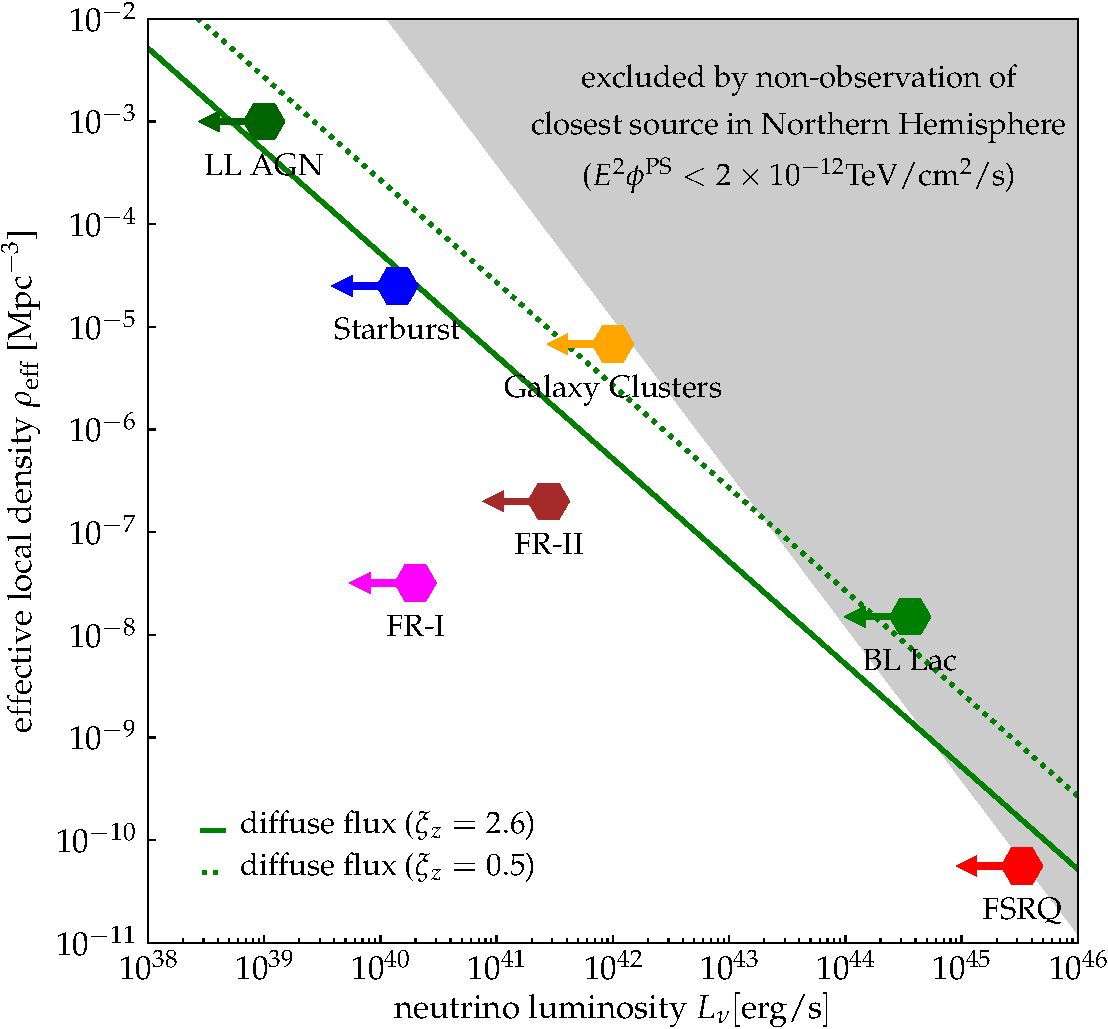
\includegraphics[width=0.5\textwidth]{figures/luminosityDISCOVERY.pdf}
\caption{Alhers Halzen~\cite{Ahlers2018ppnp}}
\label{fig:nuluminosity}
\end{figure}

\subsection{Cosmic Ray Intensity and Pion Production Rate} 

Measurements of ultra-high-energy cosmic rays (UHECRs) provide a key benchmark for understanding the production rates of secondary particles such as pions, neutrinos, and gamma rays. Observations estimate the UHECR intensity at proton energies \(E_p \gtrsim 10^{17}~\text{eV}\) as~\cite{add}:  
\begin{equation}
E_p^2 I^{\rm UHE}_p \simeq 10^{-7}~\text{GeV}~\text{cm}^{-2}~\text{s}^{-1}~\text{sr}^{-1}.
\end{equation}

From this, the corresponding cosmic-ray luminosity density is inferred as:
\begin{equation}
E_p^2 \frac{dQ_p}{dV} \simeq 10^{44}~\text{erg}~\text{Mpc}^{-3}~\text{yr}^{-1}.
\end{equation}

Using these values, we can estimate the upper limit for the pion production rate by relating it to the cosmic-ray proton production rate. The total energy production rate of pions, including both charged (\(\pi^+\)) and neutral (\(\pi^0\)), satisfies:
\begin{equation}
E_{\pi^+} Q_{\pi^+}(E_{\pi^+}) + E_{\pi^0} Q_{\pi^0}(E_{\pi^0}) \simeq \left[E_p Q_p(E_p)\right]_{E_p \simeq E_{\pi} \left\langle \frac{E_p}{E_{\pi}} \right\rangle}.
\end{equation}

To refine this relation, we use the charged-to-neutral pion production ratio \(R_\pi\), where \(Q_{\pi^+} \simeq R_\pi Q_{\pi^0}\), and the relation simplifies to:
\begin{equation}
\left(\frac{1 + R_\pi}{R_\pi}\right) E_{\pi^+} Q_{\pi^+}(E_{\pi^+}) \simeq \left[E_p Q_p(E_p)\right]_{E_p \simeq E_{\pi} \left\langle \frac{E_p}{E_{\pi}} \right\rangle}.
\end{equation}

Multiplying both sides by \(E_{\pi^+}\) gives:
\begin{equation}
\left(\frac{1 + R_\pi}{R_\pi}\right) E^2_{\pi^+} Q_{\pi^+}(E_{\pi^+}) \simeq \frac{1}{\left\langle \frac{E_p}{E_{\pi}} \right\rangle} \left[E^2_p Q_p(E_p)\right]_{E_p \simeq E_{\pi} \left\langle \frac{E_p}{E_{\pi}} \right\rangle}.
\end{equation}

Finally, we express the pion production rate as:
\begin{remark}
\begin{equation}
E^2_{\pi^+} Q_{\pi^+}(E_{\pi^+}) \simeq x_\pi \frac{R_\pi}{1 + R_\pi} \left[E^2_p Q_p(E_p)\right]_{E_p \simeq E_{\pi} \left\langle \frac{E_p}{E_{\pi}} \right\rangle},
\end{equation}
\end{remark}
where \(x_\pi\) denotes the average fraction of proton energy transferred to pions during interactions.

By integrating the production rates of secondary particles, we can determine the cumulative neutrino intensity across all flavors. The resulting neutrino intensity is given by:
\begin{equation}
\frac{1}{3} \sum_\alpha E_\nu^2 I_{\nu_\alpha} \lesssim 3 \times 10^{-8} x_\pi \left(\frac{\xi_z}{2.6}\right)~\text{GeV}~\text{cm}^{-2}~\text{s}^{-1}~\text{sr}^{-1}.
\end{equation}
Here \(x_\pi\) is the fraction of proton energy converted into pion energy, \(\xi_z \sim 2.6\) a factor accounting for redshift evolution of the sources.  

\begin{figure}[!t]
\centering
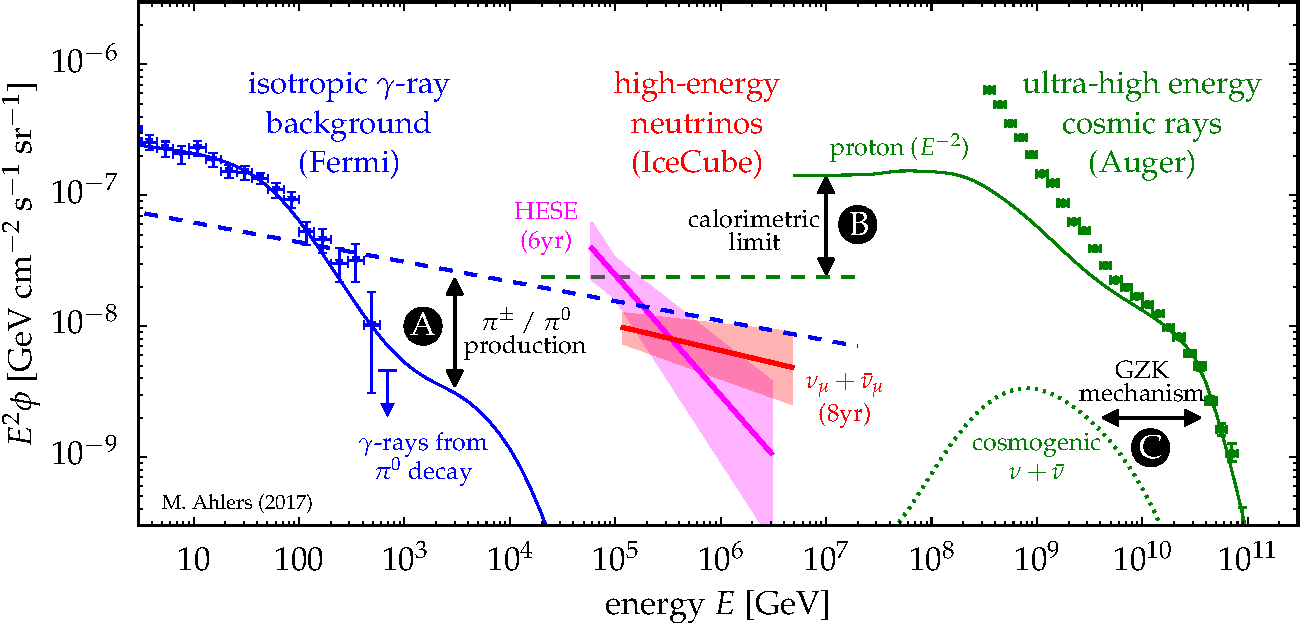
\includegraphics[width=0.90\textwidth]{figures/panorama.pdf}
\caption{Alhers Halzen~\cite{Ahlers2018ppnp}}
\label{fig:uhemm}
\end{figure}

The value \(3 \times 10^{-8}~\text{GeV}~\text{cm}^{-2}~\text{s}^{-1}~\text{sr}^{-1}\) represents the \emph{Waxman-Bahcall bound}~\cite{aaa}, also known as the calorimetric limit (see~\ref{fig:uhemm}).  

The Waxman-Bahcall bound assumes that all proton energy is efficiently converted into pions and subsequently into neutrinos. For that reason, this bound is applicable to \emph{transparent sources}, where interactions with radiation and matter inside the source allow neutrinos to escape without significant reabsorption or secondary interactions.

In transparent sources, protons are accelerated within strong magnetic fields and interact with photons to produce pions via \(p\)-\(\gamma\) interactions. The decay of these pions produces neutrinos and gamma rays, while secondary protons and neutrons may remain confined within the source. 
%
For such sources, the neutrino flux is closely tied to the gamma-ray flux, reflecting the shared origin in pion production.

Worth noticing that an important assumption in these models is that the source spectrum of accelerated particles is steeper than \(E^{-2}\). This steepness is typical of observed cosmic-ray spectra and theoretical predictions for diffusive shock acceleration in astrophysical sources. 

In more complex astrophysical environments, the local conditions—such as photon density, magnetic field strength, and matter density—can affect the overall neutrino production and escape mechanisms. For example in opaque sources, as the recently detected NGC1068 galaxy, or if additional processes, such as \(e^+\)-\(e^-\) pair production or synchrotron cooling, can redistribute energy among secondary particles.

The connection between UHECRs, neutrinos, and gamma rays offers a compelling framework for studying the most energetic processes in the universe. Observations of the diffuse neutrino background by IceCube and measurements of UHECR intensities by Auger together place strong constraints on the properties of cosmic accelerators, advancing our understanding of multi-messenger astrophysics~\cite{}.
